\documentclass[12pt]{article}
\usepackage{graphicx} % Required for inserting images
\usepackage{tikz}  % Required for drawing the process flow diagram
\usetikzlibrary{positioning} %to position the images
\usepackage{url} % Required for formatting URLs in bibilography
\usepackage[hidelinks]{hyperref} % Required for hyperlinks in bibilography
\usepackage{dirtree} % Required for directory structure

\usetikzlibrary{shapes, arrows} % Required for flowchart shapes and arrows
\tikzstyle{box}     = [rectangle, draw, fill=blue!10,
                        minimum width=3cm, minimum height=0.8cm]
\tikzstyle{arrow}   = [thick, ->, >=stealth]

\title{Report}
\author{Prajwal and Vishesh}
\date{\today}

\begin{document}

\maketitle
\tableofcontents
\clearpage
\section{Design and Architecture}
The design of the project is pretty simple, straightforward and a block based approach. \\
The authentication into the game is handled by \texttt{main.sh} which takes usernames and passwords and manage them in users.tsv file.\\
After authentication, the \texttt{game.py} is called which has the main code for the games, it has a generic class which is inherited by the three games- tic tac toe, connect four and othello.\\
The game.py has funcions common in all games such as check win, change turn, current turn player,update history, etc.\\
It also has some extra functions such as pregame countdown animation, postgame graph update, etc. which are intended for enhancing the UI and design of the game hub. These could have been added in the individual game files, but were added in the general class for code reusability. Hence most of the code possible is tried to be kept in the main file itself.\\
Other function specific to games are written in the respective game classes, the game files also import the general class.\\

\section{External Libraries Used}
\begin{itemize}
    \item pygame -ce
    \item numpy
    \item matplotlib
    \item sys
    \item os
    \item pathlib
    \item time
    \item datetime
    \item subprocess
\end{itemize}
\clearpage
\section{Installation and setup}
installed python and all the libraries mentioned in "libraries used section".\\
setup on github (made an account on github website).\\
code editors used generally - vs code, overleaf.

\section{Directory structure}


\dirtree{%
.1 hub.
.2 {Fonts and Audio}.
%.3 8-Bit-Indigestion.mp3.
%.3 PressStart2P-Regular.ttf.
.2 Games.
.3 pycache.
.3 connect4.py.
.3 othello.py.
.3 tictactoe.py.
.2 Images.
.2 Report.
.3 Makefile.
.3 Report.pdf.
.3 Report.tex.
.3 references.bib.
.2 {firework frames}.
.2 game.py.
.2 history.csv.
.2 leaderboard.sh.
.2 main.sh.
.2 users.tsv.
}
\clearpage

\section{Launching the game(Usage)}
After getting all the libraries, you can run the game by running \texttt{main.sh} in terminal, it will ask for login or registration of two players, then it will ask to select the game and then it will run the python script.\\
Basic process flow diagram of the game is as follows-\\
\begin{center}
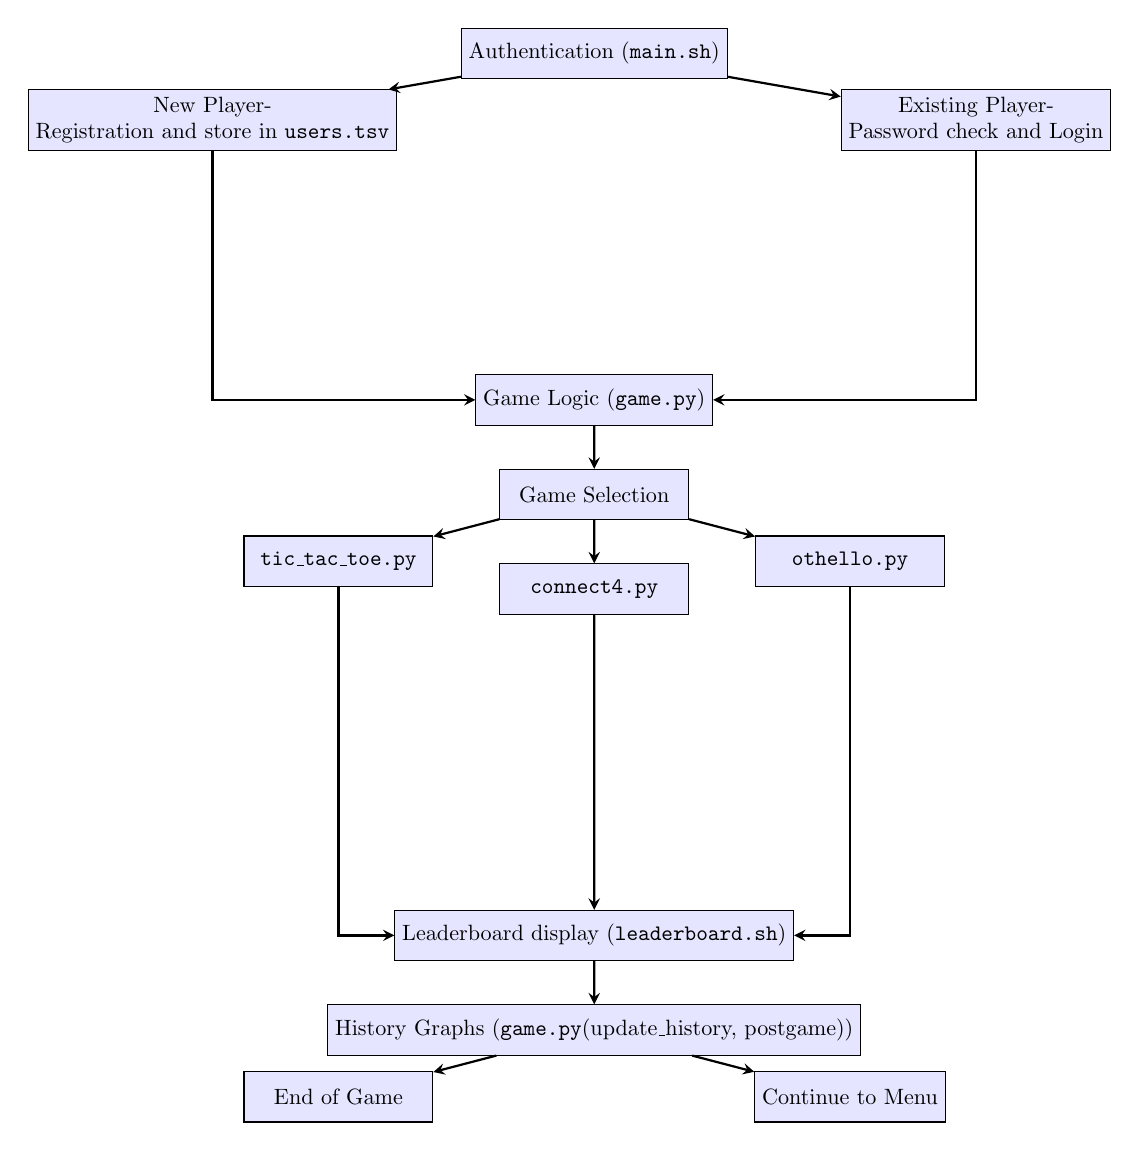
\begin{tikzpicture}[scale=0.8, transform shape, node distance=1.5cm]
\node (auth) [box] {Authentication (\texttt{main.sh})};
\node (new player) [box, below left of=auth, xshift=-5cm] {\shortstack{New Player-\\ Registration and store in \texttt{users.tsv}}};
\node (existing player) [box, below right of=auth, xshift=5cm] {\shortstack{Existing Player-\\ Password check and Login}};
\node (menu) [box, below of=auth, yshift=-4cm] {Game Logic (\texttt{game.py})};
\node (game selection) [box, below of=menu] {Game Selection};
\node (tic tac toe) [box, below left of=game selection, xshift=-3cm] {\texttt{tic\_tac\_toe.py}};
\node (connect four) [box, below of=game selection] {\texttt{connect4.py}};
\node (othello) [box, below right of=game selection, xshift=3cm] {\texttt{othello.py}};
\node (leaderboard) [box, below of=menu, yshift=-7cm] {Leaderboard display (\texttt{leaderboard.sh})};
\node (history) [box, below of=leaderboard] {History Graphs (\texttt{game.py}(update\_history, postgame))};
\node (end) [box, below left of=history, xshift=-3cm] {End of Game};
\node (continue) [box, below right of=history, xshift=3cm] {Continue to Menu};
\draw [arrow] (auth) -- (new player);
\draw [arrow] (auth) -- (existing player);
\draw [arrow] (new player) |- (menu);
\draw [arrow] (existing player) |- (menu);
\draw [arrow] (menu) -- (game selection);
\draw [arrow] (game selection) -- (tic tac toe);
\draw [arrow] (game selection) -- (connect four);
\draw [arrow] (game selection) -- (othello);
\draw [arrow] (tic tac toe) |- (leaderboard);
\draw [arrow] (connect four) -- (leaderboard);
\draw [arrow] (othello) |- (leaderboard);
\draw [arrow] (leaderboard) -- (history);
\draw [arrow] (history) -- (end);
\draw [arrow] (history) -- (continue);
\end{tikzpicture}
\end{center}
\section{Images}
\begin{figure}[h]
    \centering
    
\includegraphics[width=0.4\textwidth]{../images/pdf_images/WhatsApp Image 2026-04-29 at 16.53.00 (1).jpeg}
    \hspace{1cm}
    
\includegraphics[width=0.4\textwidth]{../images/pdf_images/WhatsApp Image 2026-04-29 at 16.53.00 (2).jpeg}\\
    \vspace{1cm}
    
\includegraphics[width=0.4\textwidth]{../images/pdf_images/WhatsApp Image 2026-04-29 at 16.53.00 (3).jpeg}
    \hspace{1cm}
    
\includegraphics[width=0.4\textwidth]{../images/pdf_images/WhatsApp Image 2026-04-29 at 16.53.00.jpeg}\\
    \vspace{1cm}
    \caption{Gameplay visuals -1}
\end{figure}

\begin{figure}[h]
    \centering
     
\includegraphics[width=0.4\textwidth]{../images/pdf_images/WhatsApp Image 2026-04-29 at 16.53.01 (1).jpeg}
    \hspace{1cm}
    
\includegraphics[width=0.4\textwidth]{../images/pdf_images/WhatsApp Image 2026-04-29 at 16.53.02.jpeg}\\
    \vspace{1cm}
    
\includegraphics[width=0.4\textwidth]{../images/pdf_images/WhatsApp Image 2026-04-29 at 16.53.01 (2).jpeg}
    \hspace{1cm}
    
\includegraphics[width=0.4\textwidth]{../images/pdf_images/WhatsApp Image 2026-04-29 at 16.53.01.jpeg}
    \caption{Gameplay visuals -2}
\end{figure}
\clearpage
\section{Features}

There are various Features we added to make the gameplay more interesting and engaging, such as-

\begin{itemize}
    

\item user authentication system using SHA-256 hashing and tsv file storage
\item multiplayer(2 player) games
\item shows history of the players wins and losses
\item uses graphs, etc to show data
\item display of characters in menu with thier player names written below them
\item background music in the game
\item falling animation of the circle in Connect Four
\item sound effects for various actions such as clicking, etc
\item background images which makes it look more attractive
\item extra animation before start of each game
\item added fireworks animation at the end of the game screen -\\ It is a loop of frames which initiate randomly and show the animation. Based on random generation and frzme shifting.

\end{itemize}
\clearpage

\section{Code Logic}

\subsection{Generic Class}
here, the code written is the parent code which is inherited by the three games, it has some functions and variables defined,such as-\\

Variables-\\
player1 and player2 stored in players array, current turn, board\\

Functions- \\
check win, current turn player, change turn\\

all these are working as thier name suggests, easy to understand\\
\\
There are also functions about Updating History, Postgame update in the graphs using history.csv as data and pregame countdown screen animations using loops and loading multiple images.\\
Generally all games have similar logic- run in loop, each time taking events and executing, updating the board array, for this calling some general functions like update board, change turn, current turn player, etc.
Hence, for each game, only unique logics are explained below
\subsection{Tic Tac Toe}
for check win, we first check the rows, then colomns, then diagonal and anti diagonals
for this i made a set of all 5*5 submatrices, then checked these conditions for each matrice
\subsection{Connect Four}
same logic as tic tac toe, just the difference is here we can add new piece only at lowest available space in colomn

%write about the logic of adding falling animation
\subsection{Othello}
a very interesting logic is used here to know if the clicked cell is valid or not. 
i made a list of 8 vectors in the 8 directions( the north south east west and the in between 45 degrees)

then at the clicked position, for each direction, i moved in that direction from the clicked position one by one in that direction checking.
if its true for all directions- found a piece of same color with the previous step color bieng opposite color
then its valid

the check win is called when no valid move is left, which simply counts the nmber of pieces of the players and returns who won


\subsection{Authentication System}
%Vishesh
The main.sh is the way to authentication in this project.The script handles login or registrations of players before launching the game. For each player, it reads a username and password, hashes the password with SHA-256, and checks it against users.tsv. New users get prompted to register with a password of at least 7 characters, returning users just get verified, and wrong passwords loop back to retry. Once both players are authenticated, their usernames are passed straight to game.py.
\subsection{Leaderboard}
%Vishesh
The Leaderboard.sh Code uses awk command to read history.csv.\\ The awk command uses associative array to count about wins losses and win/loss ratio (equal to wins of p if losses is 0). Using formatted printing the table is printed for all games using a loop.\\  Another task is to print according to different metrics. For this we pass the metrics as an argument for the bash script. According to that argument an appropriate piped sort command does the sorting for the leaderboard table.\\
Later the Leaderboard data funcion uses the history.csv and leaderboard to make a bar graph and pie chart using MatPlotLib.

\clearpage

\section{Retrospective}
\subsection{axis}
it was very difficult for us to understand the concept of axis, we tried a lot of things - reading documents, watched videos but still it wasnt clear visually.\\

Solution-i came up with a concept/theory which was working all the time.
it is that for a vector of dimension=n, axis=k represent a set of the groups. (a group is the set of of those elements who have all indices identical except the kth indice.)

\subsection{Othello's logic}
it was too confusing that how can i make othello without using for loops , also it was difficult to check a valid move ...
\\
Solution- it was later announced that except in check win function, we can use for loops, also i came up with an idea of the 8 direction vectors checking.

\subsection{diagonal check win}
since tic tac toe was 10*10, to check win the diagonals, it was so difficult to check the non-main diagonals without using for loop.
\\
Solution-i got an idea that instead i can just check the 5*5 squares because here i wont have to check non main diagonals in 5*5, hence i made a set of all 5*5 squares and simplified it.
\subsection{Text alignment with varying length of player names}
it was difficult to align the text of player names with the character images in menu because the length of player names can vary and hence the text can be misaligned, which will affect the look of UI.
\\
Solution- I defined a rectangle box for the text(using \texttt{pygame.getRect}) and aligned the text in the center of that box, hence no matter what the length of the text is, it will always be aligned in the center of the box and hence with the character image.
\subsection{Arrangement according to the background image for various games}
it was difficult to arrange the figures etc according to the background image for various games, because each game has different background image and hence the arrangement for one game may not look good for another game.
\\
Solution- I made different arrangements for each game according to the background image by manually checking the offsets and side lengths, and also made some general arrangements which can be used in all games, such as the arrangement of player names and scores, etc.
%you can add your hurdles...
\clearpage
\section{What would we do with 10 more hours}
\subsection{Add new games}
With 10 more hours, we could add one more board game like checkers, chess,e.t.c.
there are various such game ideas available on 2 players, a mobile game
\subsection{Make better UI}
We could make a better UI like better sound effects, background picture, background music etc.
add more animations, try to increase smoothness in animations
\subsection{Optimise}
We could optimise our existing code so that it could run faster, use lesser memory
\subsection{Add settings}
We could add settings option in menu, in which user can control various things like volume, e.t.c.
\clearpage

%add bibilography and citations
\nocite{*}
\bibliographystyle{plain}
\bibliography{references}
\end{document}
